\documentclass{beamer}
\usepackage[utf8]{inputenc}
\usepackage[serbian]{babel}
\usetheme{Berlin}

\title{Korisni alati za programiranje Android aplikacija}
\author{   Danilo Nikolaš, mi21112@alas.matf.bg.ac.rs,
	\\ Luka Nedeljković, mi21147@alas.matf.bg.ac.rs,
	\\ Nemanja Kelečević, mi21071@alas.matf.bg.ac.rs,
	\\ Ivan Vlahović, mi21266@alas.matf.bg.ac.rs}
\institute[]{Matematički fakultet, Univerzitet u Beogradu}
\date{
	\footnotesize{Beograd, 2022.}	
}

\begin{document}
\begin{frame}
	\titlepage
\end{frame}


\begin{frame}
	\frametitle{Sadržaj}
	\tableofcontents[hidesubsections] 
\end{frame}

\begin{frame}
    \section{Uvod}
    \frametitle{Uvod} 
    \begin{itemize}
	\item Android programiranje
	\item Okruženja za razvoj Android aplikacija
	\item Android Studio, Unity3D, Appcelerator i Basic4Android
   \end{itemize}
\end{frame}

\begin{frame}
    \section{Android Studio}
    \frametitle{Android Studio} 
    \begin{itemize}
	\item Integrisano razvojno okruženje, zasnovano na programskog jeziku Java.
	\item Poseduje veliki broj alata koji programeri mogu da koriste.
	\item  Može se koristiti za sve Android uređaje.
   \end{itemize}
   \begin{figure}[ht!]
    \centering
    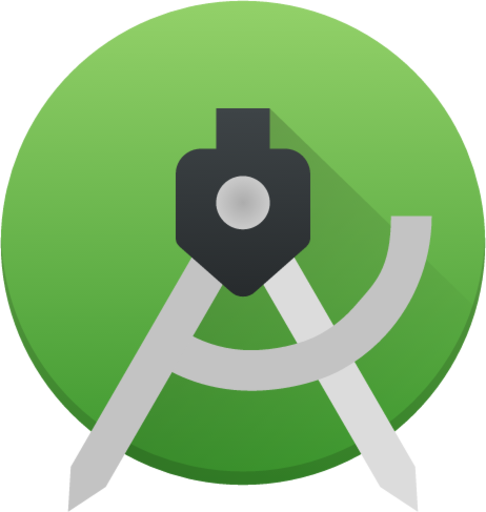
\includegraphics[scale=0.10]{android_studio_logo.png}
\end{figure}
\end{frame}

\begin{frame}
    \frametitle{AVD Manager i Android Debug Bridge}

\begin{figure}
    \centering
    \begin{minipage}{.5\textwidth}
    \centering
    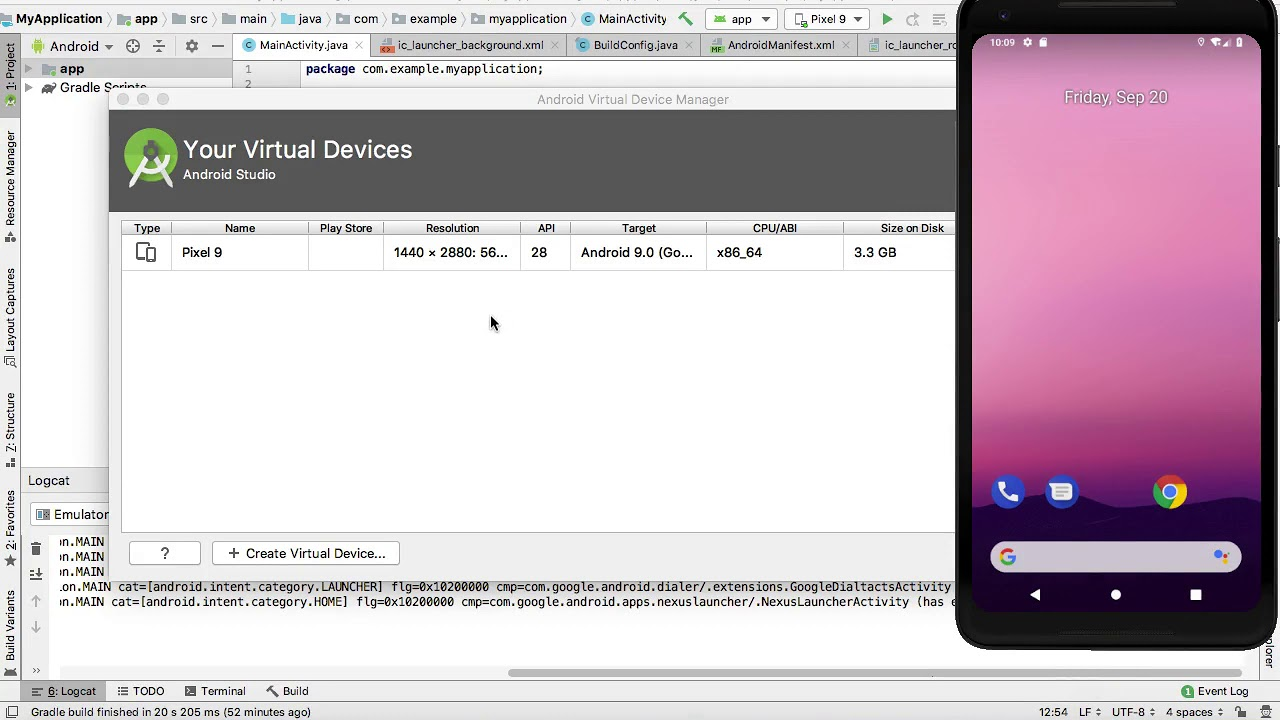
\includegraphics[width=0.9\linewidth]{avd_manager.jpg}
    \caption{AVD Manager}
    \end{minipage}%
    \begin{minipage}{.5\textwidth}
    \centering
    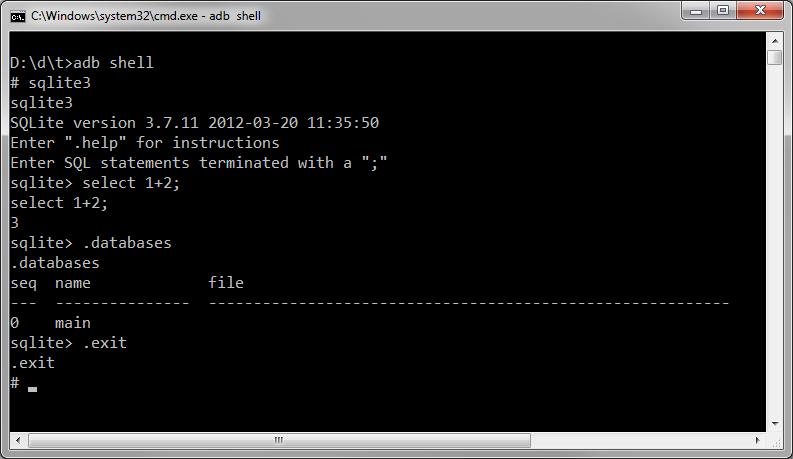
\includegraphics[width=0.8\linewidth]{adb.png}
    \caption{Android Debug Bridge}
    \end{minipage}
\end{figure}

\end{frame}

\begin{frame}
    \section{Unity 3D}
    \frametitle{Unity 3D} 
    \begin{itemize}
	\item Višeplatformsko okruženje za razvoj igara sa ugrađenim razvojnim okruženjem. 
        \item Prvobitno dizajniran za Mac računare, kasnije razvijen na mnogim platformama. 
	\item C# kao primarni programski jezik Unity-a.
	\item Jednostavan, intuitivan i prilagodljiv interfejs.
        \item Unity ima široku primenu na velikom broju platformi.
	\item Asset Store - mesto na kom programeri dele svoje kodove i biblioteke. 
   \end{itemize}
\end{frame}

\begin{frame}
    \section{Appcelerator}
    \frametitle{Appcelerator} 
    \begin{itemize}
    	\item Razvojni program za više platforme.
	\item Kompatibilan za Windows, Android i iOS.
	\item ,,Sve što nam je potrebno za kreiranje izvornih aplikacija za mobilne uređaje - iz jedne osnove JavaScript koda".
	\item  Titanium - platforma za razvoj.
   \end{itemize}
\end{frame}

\begin{frame}
    \section{Basic4Android}
    \frametitle{Basic4Android} 
    \begin{itemize}
	\item Alatka za brzi razvoj aplikacija na Androidu.
	\item B4I - alatka za brzi razvoj aplikacija na iOS-u.
	\item Alternativa programiranju u Javi.
   \end{itemize}
\end{frame}

\begin{frame}
    \section{Zaključak}
    \frametitle{Zaključak} 
    \begin{itemize}
	\item Android je projekat koji mnogo obećava.
	\item Zajednica otvorenog koda omogućuje brz napredak.
	\item Okruženja koja koristimo za razvoj Android aplikacija igraju veoma značajnu ulogu.
	
   \end{itemize}
\end{frame}

\begin{frame}
    \frametitle{Literatura}
    \begin{itemize}
    	\item Unity 3D - https://www.mindinventory.com/blog/unity-3d-game-development/
	\item Appcelerator - https://bs.eyewated.com/top-5-alatki-za-razvoj-multiformnih-mobilnih-aplikacija/
	\item Alati za programere - https://www.androidsis.com/bs/najbolji-alati-za-programere-android-aplikacija/
	\item Android Studio - https://androidayuda.com/bs/android-studio/
   \end{itemize}
\end{frame}

\end{document}
